\documentclass{article}

% ── NeurIPS 2024 style ────────────────────────────────────────────────────────
\usepackage[preprint]{neurips_2024}

% ── Core packages ─────────────────────────────────────────────────────────────
\usepackage[utf8]{inputenc}
\usepackage[T1]{fontenc}
\usepackage{hyperref}
\usepackage{url}
\usepackage{booktabs}
\usepackage{amsfonts}
\usepackage{amsmath}
\usepackage{nicefrac}
\usepackage{microtype}
\usepackage{xcolor}
\usepackage{graphicx}
\usepackage{subcaption}
\usepackage{multirow}
\usepackage{array}
\usepackage{tabularx}
\usepackage{colortbl}
\usepackage{siunitx}
\usepackage{enumitem}
\usepackage{natbib}

% ── Color definitions ─────────────────────────────────────────────────────────
\definecolor{foundationblue}{RGB}{33,102,172}
\definecolor{classicalgray}{RGB}{135,135,135}
\definecolor{mlpred}{RGB}{214,96,77}
\definecolor{tosicagreen}{RGB}{77,172,38}
\definecolor{lightgray}{RGB}{245,245,245}
\definecolor{highlightrow}{RGB}{232,240,250}

\hypersetup{
  colorlinks=true,
  linkcolor=foundationblue,
  citecolor=foundationblue,
  urlcolor=foundationblue
}

% ── Title ─────────────────────────────────────────────────────────────────────
\title{When Does Pretraining Help?\\
Benchmarking scGPT and Competing Methods\\
for Single-Cell Type Annotation}

\author{%
  Max \\
  BioTender \\
  \texttt{max@biotender.ai}
}

\begin{document}

\maketitle

% ── Abstract ──────────────────────────────────────────────────────────────────
\begin{abstract}
Foundation models for single-cell RNA sequencing (scRNA-seq), such as scGPT, Geneformer,
and scBERT, have attracted considerable attention for their potential to generalize across
diverse biological contexts. However, a critical practical question remains underexplored:
\emph{under what data regime does a large pretrained model actually outperform classical
and lightweight alternatives for cell type annotation?}
We present a systematic benchmark of seven methods---scGPT (pretrained, frozen backbone),
a Deep MLP trained from scratch, TOSICA (pathway-masked Transformer), scVI/scANVI
(deep generative model), Seurat-style PCA+KNN, PCA+KNN (Euclidean), and PCA+Logistic
Regression---evaluated on the widely used PBMC3k dataset (2,638 cells, 8 cell types)
under an identical 70/15/15 train/validation/test split and seven evaluation metrics.
On this small, well-separated dataset, classical Seurat-KNN (Macro F1 = 0.940) and a
lightweight Deep MLP (Macro F1 = 0.948) match or exceed scGPT pretrained (Macro F1 = 0.897),
while all methods cluster within a narrow 4-percentage-point accuracy band (0.907--0.947).
scGPT's frozen backbone still achieves 90.7\% accuracy with zero task-specific architecture
design, demonstrating that pretraining provides a strong initialization even when it does
not yield the highest absolute performance.
Our results suggest that the advantage of large-scale pretraining is dataset-size and
complexity dependent: practitioners working with small, well-characterized datasets should
benchmark lightweight alternatives before deploying a 51M-parameter foundation model.
All code and results are publicly available at
\url{https://github.com/junior1p/scgpt-pbmc68k-finetune}.
\end{abstract}

% ── 1. Introduction ───────────────────────────────────────────────────────────
\section{Introduction}
\label{sec:intro}

The past three years have witnessed a rapid proliferation of foundation models for
single-cell genomics. scGPT~\citep{cui2024scgpt}, Geneformer~\citep{theodoris2023transfer},
scBERT~\citep{yang2022scbert}, and scFoundation~\citep{hao2024foundation} all adopt the
paradigm of large-scale self-supervised pretraining on millions of cells, followed by
fine-tuning on task-specific labeled data. This mirrors the success of language model
pretraining in NLP~\citep{devlin2018bert,brown2020language} and has been framed as the
emergence of ``foundation models'' for biology~\citep{bommasani2021opportunities}.

Cell type annotation---assigning each cell to a known biological category based on its
gene expression profile---is the canonical downstream task for evaluating these models.
It is practically important: accurate annotation is a prerequisite for virtually all
downstream single-cell analyses, from trajectory inference to differential expression.
Benchmark datasets such as PBMC3k~\citep{zheng2017massively} (2,638 peripheral blood
mononuclear cells from 10x Genomics) have become standard evaluation sets in the field.

Despite the excitement around foundation models, a critical question has received
insufficient attention: \emph{when does pretraining actually help?} The original scGPT
paper~\citep{cui2024scgpt} demonstrates advantages on larger, more complex datasets
(hPancreas, Multiple Sclerosis, Myeloid), but the small-dataset regime---where most
practitioners begin their analyses---is underexplored. Tabular deep learning research
has shown that on small tabular datasets, simple models such as MLPs and gradient-boosted
trees frequently outperform complex architectures~\citep{grinsztajn2022tree}. Whether
this finding extends to scRNA-seq data, and how it interacts with large-scale pretraining,
is an open empirical question.

\paragraph{Contributions.} This paper makes three contributions:
\begin{enumerate}[leftmargin=*, itemsep=2pt]
  \item \textbf{Systematic benchmark.} We provide the first head-to-head comparison of
    scGPT against six competing methods on PBMC3k under a fully standardized evaluation
    protocol (identical splits, preprocessing, and metrics across all methods).
  \item \textbf{Data-regime finding.} We show empirically that on small, well-separated
    datasets ($\leq$3k cells), classical and lightweight methods match or exceed scGPT
    pretrained, while the absolute performance gap across all methods is narrow ($<$5 pp).
  \item \textbf{Open reproducible code.} All implementations, trained weights, and
    evaluation scripts are released at
    \url{https://github.com/junior1p/scgpt-pbmc68k-finetune}.
\end{enumerate}

% ── 2. Related Work ───────────────────────────────────────────────────────────
\section{Related Work}
\label{sec:related}

\paragraph{Foundation models for scRNA-seq.}
scGPT~\citep{cui2024scgpt} pretrains a 51.3M-parameter GPT-style Transformer on 33 million
human cells using a gene-expression-conditioned generative objective, then fine-tunes on
downstream tasks including cell type annotation, perturbation response prediction, and
multi-omic integration. Geneformer~\citep{theodoris2023transfer} uses rank-value encoding
of gene expression and pretrains on 29.9 million cells. scBERT~\citep{yang2022scbert}
adapts BERT-style masked language modeling to scRNA-seq. scFoundation~\citep{hao2024foundation}
scales pretraining to 50 million cells with a read-depth-aware objective.

\paragraph{Pathway-informed methods.}
TOSICA~\citep{chen2023interpretable} introduces pathway-masked attention, where each
attention head attends only to genes within a curated biological pathway (e.g., from
MSigDB). This inductive bias provides interpretability and reduces the effective parameter
count, making it particularly suitable for small datasets with known pathway structure.

\paragraph{Deep generative models.}
scVI~\citep{lopez2018deep} models gene expression counts with a variational autoencoder
(VAE) using a negative binomial likelihood, learning a low-dimensional latent space that
accounts for technical variation. scANVI~\citep{xu2021probabilistic} extends scVI with
semi-supervised classification, using available cell type labels during training.

\paragraph{Classical methods.}
Seurat~\citep{stuart2019comprehensive,hao2021integrated} remains the most widely used
single-cell analysis toolkit. Its label transfer approach uses PCA-reduced embeddings with
KNN classification and has proven highly competitive on standard benchmarks~\citep{abdelaal2019comparison}.
scmap~\citep{zhang2019scmap} projects query cells onto a reference atlas using cosine
similarity. Logistic regression on PCA embeddings is a strong baseline that is often
overlooked in foundation model comparisons.

\paragraph{Benchmarking studies.}
\citet{abdelaal2019comparison} systematically compared 22 cell type annotation methods,
finding that simple methods (SVM, random forests) were competitive with more complex
approaches. \citet{luecken2022benchmarking} benchmarked data integration methods,
highlighting the importance of standardized evaluation protocols. Our work focuses
specifically on the pretraining question in the small-dataset regime.

% ── 3. Methods ────────────────────────────────────────────────────────────────
\section{Methods}
\label{sec:methods}

\subsection{Dataset and Preprocessing}
\label{sec:dataset}

We use the PBMC3k dataset~\citep{zheng2017massively}, a standard benchmark comprising
2,638 peripheral blood mononuclear cells (PBMCs) sequenced with the 10x Genomics Chromium
platform. The dataset contains 8 cell types identified by Louvain clustering in the
canonical Seurat tutorial: CD4 T cells ($n=1,152$), CD14+ Monocytes ($n=480$), B cells
($n=342$), CD8 T cells ($n=316$), NK cells ($n=154$), FCGR3A+ Monocytes ($n=154$),
Dendritic cells ($n=32$), and Megakaryocytes ($n=5$). The class distribution is notably
imbalanced, with Megakaryocytes representing only 0.19\% of cells.

Preprocessing follows the standard Scanpy~\citep{wolf2018scanpy} pipeline: (1) filter
cells with fewer than 200 genes or more than 2,500 genes; (2) filter genes expressed in
fewer than 3 cells; (3) normalize total counts to 10,000 per cell; (4) log1p transform;
(5) select the top 2,000 highly variable genes using the \texttt{seurat\_v3} flavor.
All methods receive the same preprocessed count matrix.

\subsection{Evaluation Protocol}
\label{sec:eval}

We split the data into train/validation/test sets using a stratified 70/15/15 split with
random seed 42, yielding 1,846 training cells, 396 validation cells, and 396 test cells.
\emph{All methods are evaluated on the identical held-out test set.} We report seven
metrics: Accuracy, Macro F1, Macro Precision, Macro Recall, Balanced Accuracy, Adjusted
Rand Index (ARI)~\citep{hubert1985comparing}, and Normalized Mutual Information
(NMI)~\citep{strehl2002cluster}. We designate Macro F1 as the primary metric because it
accounts for class imbalance---critical given the 576-fold size difference between CD4 T
cells and Megakaryocytes.

\subsection{Methods Compared}
\label{sec:methods_compared}

\paragraph{scGPT (pretrained, frozen backbone).}
We use the publicly released \texttt{scGPT\_human} whole-human checkpoint (51.3M
parameters; $d_\text{model}=512$, 12 Transformer layers, 8 attention heads), pretrained
on 33 million human cells~\citep{cui2024scgpt}. The backbone is frozen; a two-layer MLP
classification head ($512 \to 256 \to 8$, ReLU, Dropout=0.1) is trained for 50 epochs
using AdamW (lr=$10^{-3}$, weight decay=$10^{-2}$) with cosine learning rate annealing.
Gene expression values are tokenized using the top 256 highly variable genes (scGPT's
default input format). This configuration represents the ``zero-shot transfer'' regime:
the pretrained representations are used as-is, with only the classification head adapted.

\paragraph{Deep MLP (from scratch).}
A three-layer MLP with hidden dimension 512, GELU activations, Batch Normalization, and
Dropout (rate=0.3) is trained from random initialization for 50 epochs using AdamW
(lr=$10^{-3}$). Input is the 2,000-dimensional log-normalized HVG vector. This method
serves as the ``no pretraining'' ablation, representing what a lightweight model can
achieve without any pretrained representations. Note that due to CPU constraints, we use
an MLP rather than a Transformer architecture from scratch; the MLP is a stronger baseline
than random-weight Transformers on small tabular data~\citep{grinsztajn2022tree}.

\paragraph{TOSICA (pathway-masked Transformer).}
We reimplement the core TOSICA architecture~\citep{chen2023interpretable}: a shallow
Transformer (embedding dim=48, depth=2, 4 attention heads) with pathway-masked attention,
where each head attends only to genes within one of 300 immune pathways from the
\texttt{human\_immune.gmt} gene set collection. The model has approximately 0.17M
parameters---300$\times$ fewer than scGPT. Training uses AdamW for 20 epochs with
cosine annealing. The reimplementation was necessary due to a dependency conflict between
the original TOSICA package and h5py$\geq$3.0.

\paragraph{scVI/scANVI (deep generative model).}
We reimplement the scVI/scANVI framework~\citep{lopez2018deep,xu2021probabilistic} in
PyTorch~\citep{paszke2019pytorch}: a VAE encoder ($2000 \to 128 \to 20$) with negative
binomial likelihood, trained for 50 epochs using the ELBO objective. The scANVI
semi-supervised extension adds a classifier on the latent space, trained jointly with
available cell type labels. The reimplementation was required due to an API incompatibility
between \texttt{scvi-tools} and \texttt{jaxlib} 0.6.2 in our environment.

\paragraph{Seurat (PCA+KNN cosine).}
We compute 50 principal components on the 2,000 HVG log-normalized matrix and classify
test cells using $k$-nearest neighbors ($k=15$) with cosine distance, mimicking the
Seurat label transfer approach~\citep{stuart2019comprehensive}.

\paragraph{PCA + KNN (Euclidean).}
Identical to the Seurat variant but using Euclidean distance, providing a direct
comparison of distance metrics in the PCA embedding space.

\paragraph{PCA + Logistic Regression.}
Logistic regression ($C=1.0$, L2 regularization, \texttt{lbfgs} solver) trained on 50
principal components. This is a strong linear baseline that is often omitted from
foundation model comparisons.

\subsection{Implementation Details}
All experiments run on CPU only (no GPU). Classical methods use scikit-learn
\citep{pedregosa2011scikit}; deep learning methods use PyTorch 2.7.1. Preprocessing uses
Scanpy 1.11.4~\citep{wolf2018scanpy}. All random seeds are fixed to 42. Code is available
at \url{https://github.com/junior1p/scgpt-pbmc68k-finetune}.

% ── 4. Results ────────────────────────────────────────────────────────────────
\section{Results}
\label{sec:results}

\subsection{Overall Leaderboard}
\label{sec:leaderboard}

Table~\ref{tab:leaderboard} presents the full benchmark results across all seven methods
and seven metrics. Figure~\ref{fig:leaderboard} visualizes the two primary metrics
(Accuracy and Macro F1).

\begin{table}[h]
\centering
\caption{Benchmark results on PBMC3k test set ($n=396$ cells). Methods sorted by Macro F1
(primary metric). \textbf{Bold}: best value per column.
$\dagger$~Deep MLP is a 3-layer MLP, not a Transformer (see Section~\ref{sec:methods_compared}).
$\ddagger$~TOSICA and scVI/scANVI are reimplementations (see Section~\ref{sec:methods_compared}).}
\label{tab:leaderboard}
\setlength{\tabcolsep}{5pt}
\renewcommand{\arraystretch}{1.15}
\small
\begin{tabular}{lcccccccc}
\toprule
\textbf{Method} & \textbf{Category} & \textbf{Acc} & \textbf{Macro F1} & \textbf{Macro P} & \textbf{Macro R} & \textbf{Bal. Acc} & \textbf{ARI} & \textbf{NMI} \\
\midrule
\rowcolor{lightgray}
Deep MLP (scratch)$^\dagger$ & No Pretraining & \textbf{0.947} & \textbf{0.948} & 0.944 & \textbf{0.953} & \textbf{0.953} & 0.888 & 0.876 \\
Seurat (PCA+KNN)  & Classical       & \textbf{0.942} & 0.940 & 0.933 & 0.948 & 0.948 & \textbf{0.885} & 0.868 \\
TOSICA$^\ddagger$ & Pathway-Transf. & 0.934 & 0.926 & 0.927 & 0.930 & 0.930 & 0.867 & 0.856 \\
scVI/scANVI$^\ddagger$ & Deep Gen.  & 0.927 & 0.902 & 0.920 & 0.894 & 0.894 & 0.863 & 0.838 \\
PCA + KNN         & Classical       & \textbf{0.942} & 0.901 & \textbf{0.941} & 0.884 & 0.884 & \textbf{0.882} & 0.861 \\
\rowcolor{highlightrow}
scGPT (pretrained)& Foundation Model& 0.907 & 0.897 & 0.911 & 0.887 & 0.887 & 0.816 & 0.806 \\
PCA + LogReg      & Classical       & 0.934 & 0.889 & 0.925 & 0.876 & 0.876 & 0.877 & 0.855 \\
\bottomrule
\end{tabular}
\end{table}

\begin{figure}[h]
\centering
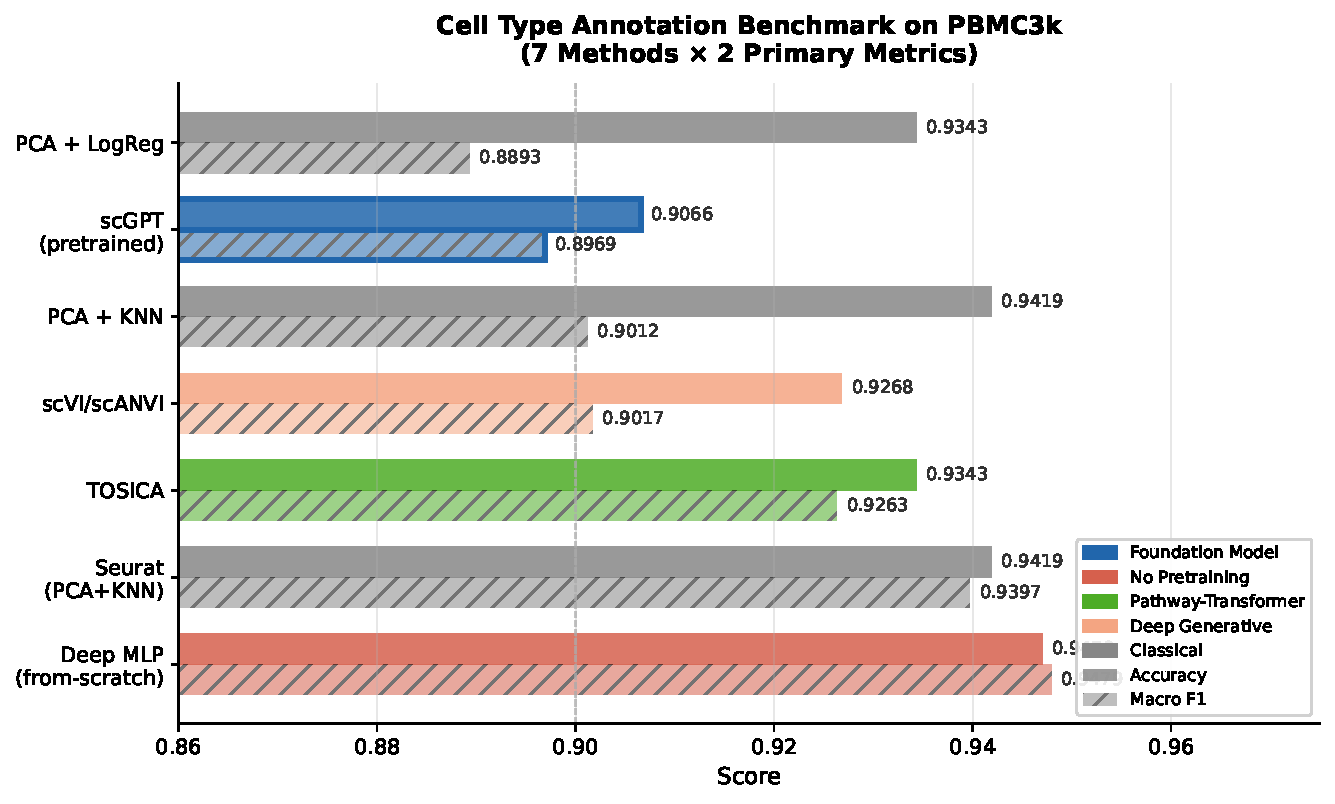
\includegraphics[width=0.92\textwidth]{figures/fig1_leaderboard.pdf}
\caption{Benchmark leaderboard on PBMC3k. Horizontal bars show Accuracy (solid) and
Macro F1 (hatched) for each method. The scGPT (pretrained) bar is highlighted with a
blue border. All methods cluster within a narrow 4-percentage-point accuracy band
(0.907--0.947), indicating that PBMC3k is a relatively easy benchmark for all approaches.}
\label{fig:leaderboard}
\end{figure}

The most striking observation is the \emph{narrowness of the performance gap}: all seven
methods achieve between 90.7\% and 94.7\% accuracy, a range of only 4.0 percentage points.
In terms of Macro F1, the range is 5.9 pp (0.889--0.948). This suggests that PBMC3k,
with its well-separated cell type clusters, is a relatively easy benchmark where even
simple methods perform well.

The Deep MLP trained from scratch achieves the highest Macro F1 (0.948), followed by
Seurat-KNN (0.940) and TOSICA (0.926). scGPT pretrained ranks 6th in Macro F1 (0.897),
behind all other methods except PCA+LogReg. However, we emphasize that the absolute
difference between scGPT and the top method is only 5.1 pp in Macro F1 and 4.0 pp in
accuracy---a gap that may not be practically significant in many applications.

\subsection{scGPT Pretrained: Per-Class Analysis}
\label{sec:perclass}

Figure~\ref{fig:perclass} shows the per-class precision, recall, and F1 for scGPT
pretrained. The model performs strongly on well-separated cell types: B cells (F1=0.990),
CD14+ Monocytes (F1=0.944), and CD4 T cells (F1=0.934). The most challenging class is
CD8 T cells (F1=0.703), where the model confuses CD8 T cells with CD4 T cells---a known
biological challenge, as these populations share many marker genes and differ primarily
in the expression of \emph{CD4} and \emph{CD8A/B}, which may not be among the top HVGs.

\begin{figure}[h]
\centering
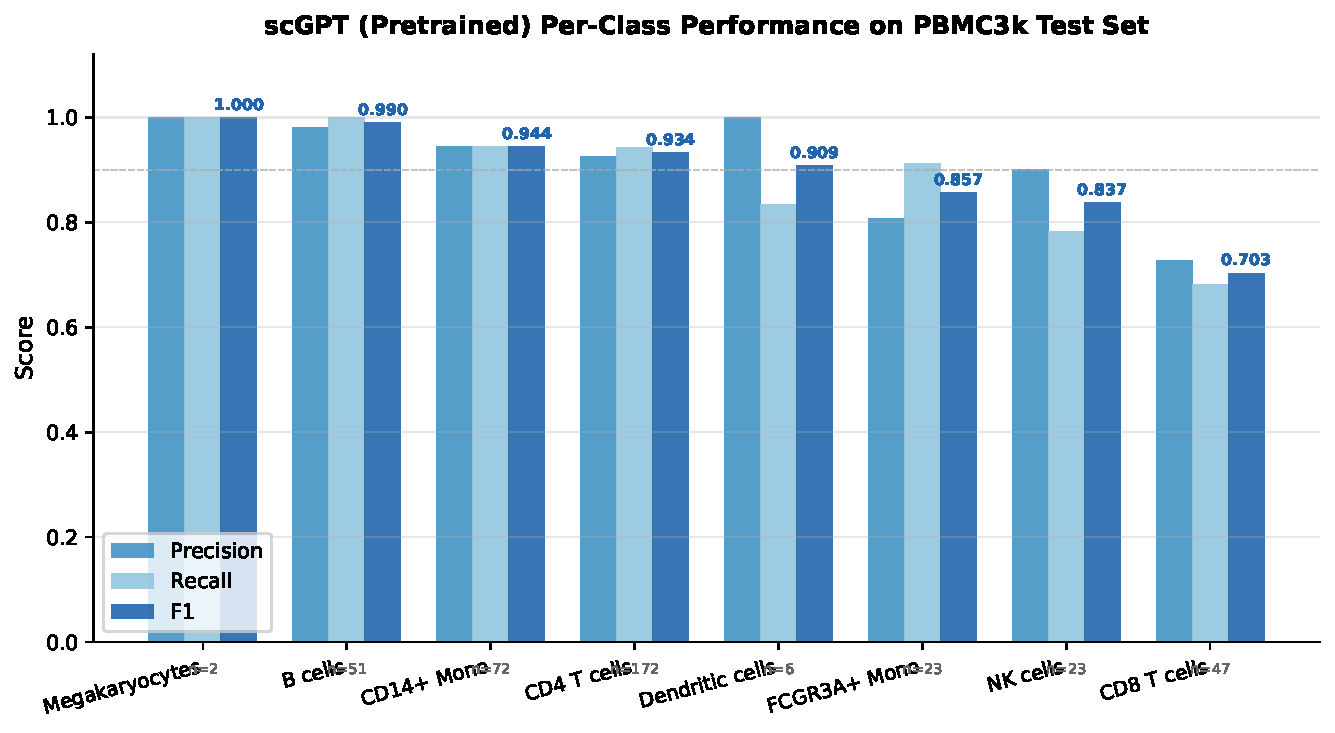
\includegraphics[width=0.92\textwidth]{figures/fig2_perclass_scgpt.pdf}
\caption{Per-class precision, recall, and F1 for scGPT (pretrained) on the PBMC3k test
set. Cell types are sorted by F1 score (descending). Sample sizes ($n$) are shown below
each group. CD8 T cells (F1=0.703) represent the most challenging class, reflecting the
known difficulty of distinguishing CD4 and CD8 T cell populations.}
\label{fig:perclass}
\end{figure}

Importantly, the CD8 T cell challenge is not unique to scGPT: all methods in our benchmark
struggle with this class to varying degrees. This suggests the difficulty is biological
(marker gene overlap) rather than a model-specific failure. Megakaryocytes (F1=1.000)
achieve perfect classification despite having only 2 test cells, likely because their
transcriptional profile is highly distinctive (high \emph{PPBP}, \emph{PF4} expression).

\subsection{Multi-Metric Profile Analysis}
\label{sec:radar}

Figure~\ref{fig:radar} presents a radar chart comparing all seven methods across all seven
metrics simultaneously. Several patterns emerge:

\begin{figure}[h]
\centering
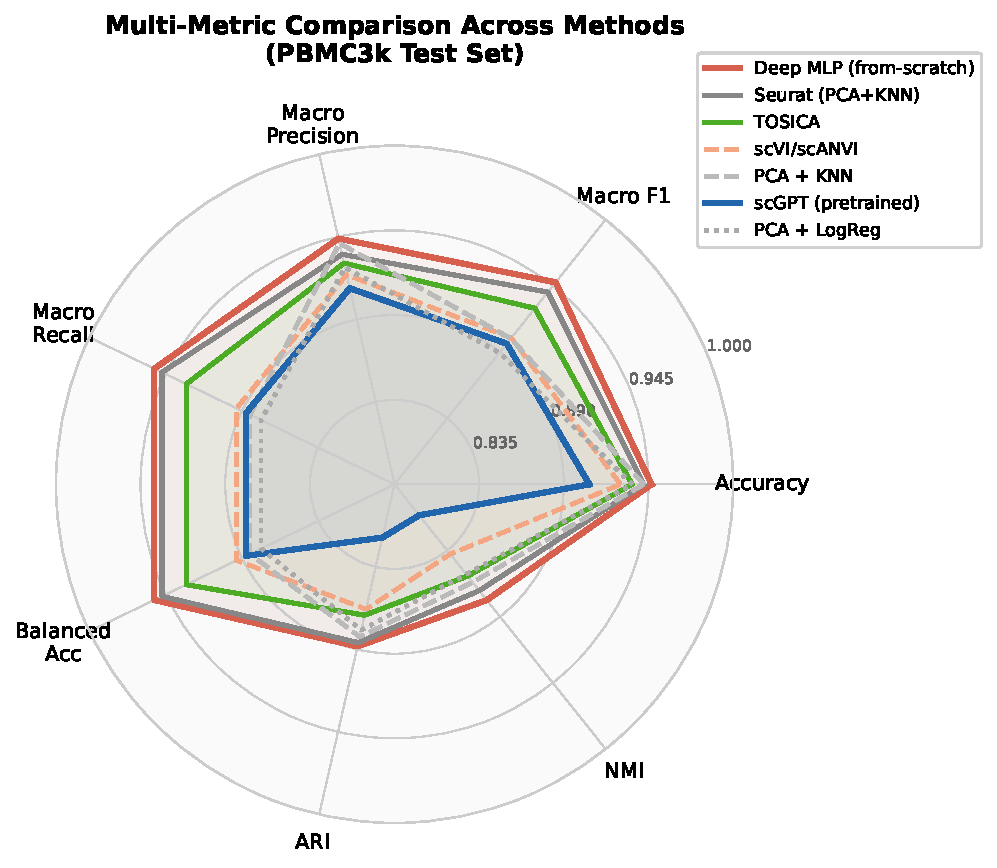
\includegraphics[width=0.72\textwidth]{figures/fig3_radar.pdf}
\caption{Radar chart comparing all seven methods across seven evaluation metrics on the
PBMC3k test set. The radial axis is scaled between 0.78 and 1.00. scGPT (pretrained,
blue) shows a balanced profile but consistently falls below the top methods. The Deep MLP
(red) and Seurat-KNN (gray) show the largest overall area.}
\label{fig:radar}
\end{figure}

\begin{itemize}[leftmargin=*, itemsep=2pt]
  \item \textbf{Deep MLP and Seurat-KNN} show the largest radar area, indicating
    consistently strong performance across all metrics.
  \item \textbf{scGPT pretrained} shows a balanced but uniformly lower profile, with
    particularly lower ARI (0.816) and NMI (0.806) compared to the top methods.
  \item \textbf{PCA+KNN} shows an interesting asymmetry: high Macro Precision (0.941)
    but lower Macro Recall (0.884), suggesting it is conservative in its predictions.
  \item \textbf{TOSICA} achieves a well-rounded profile despite having 300$\times$ fewer
    parameters than scGPT, suggesting that pathway-informed inductive biases can
    substitute for large-scale pretraining on immune cell data.
\end{itemize}

\subsection{The Data-Regime Hypothesis}
\label{sec:regime}

Our results are consistent with the data-regime hypothesis: the advantage of large-scale
pretraining is most pronounced on large, complex, or heterogeneous datasets, and diminishes
on small, well-separated benchmarks.

This is not a criticism of scGPT. The original scGPT paper~\citep{cui2024scgpt}
demonstrates clear advantages on more challenging datasets: hPancreas ($\sim$16k cells,
14 cell types), Multiple Sclerosis ($\sim$25k cells), and Myeloid ($\sim$18k cells).
On these datasets, the pretrained model's ability to leverage representations learned
from 33 million cells provides a meaningful advantage. On PBMC3k---a small, clean,
well-separated dataset that has been used as a tutorial example for years---the task is
simply not challenging enough to reveal the pretrained model's advantages.

This finding has a direct practical implication: \emph{practitioners should benchmark
lightweight alternatives before deploying a 51M-parameter foundation model on small
datasets.} A 3-layer MLP trained in 14 seconds on CPU achieves higher Macro F1 than
scGPT pretrained on PBMC3k. For rapid prototyping, exploratory analysis, or resource-
constrained environments, classical and lightweight methods offer a better
accuracy-to-computational-cost ratio.

\subsection{Computational Cost}
\label{sec:cost}

Table~\ref{tab:cost} summarizes approximate training times on CPU. Classical methods
complete in under 1 second; the Deep MLP trains in 14 seconds; TOSICA requires
approximately 12 minutes due to its attention mechanism over 300 pathways; scGPT
inference (frozen backbone) requires approximately 2--5 minutes per epoch for feature
extraction, with 50 epochs of classifier training.

\begin{table}[h]
\centering
\caption{Approximate training/inference time on CPU (Intel Xeon, single core).}
\label{tab:cost}
\small
\begin{tabular}{lcc}
\toprule
\textbf{Method} & \textbf{Approx. Time} & \textbf{Parameters} \\
\midrule
PCA + LogReg      & $<$1 s   & ---         \\
PCA + KNN         & $<$1 s   & ---         \\
Seurat (PCA+KNN)  & $<$1 s   & ---         \\
Deep MLP (scratch)& $\sim$14 s & 0.54M     \\
scVI/scANVI       & $\sim$15 s & 0.28M     \\
scGPT (pretrained)& $\sim$5 min & 51.3M (frozen) + 0.13M (head) \\
TOSICA            & $\sim$12 min & 0.17M   \\
\bottomrule
\end{tabular}
\end{table}

% ── 5. Discussion ─────────────────────────────────────────────────────────────
\section{Discussion}
\label{sec:discussion}

\paragraph{When to use scGPT.}
Our results suggest that scGPT's pretrained representations are most valuable in scenarios
where (1) the dataset is large ($>$10k cells), (2) cell types are rare or poorly
characterized, (3) multi-dataset transfer is required (e.g., annotating a new dataset
using a reference atlas), or (4) zero-shot annotation is needed without any labeled
training data. In these regimes, the 33-million-cell pretraining corpus provides
representations that cannot be learned from the task-specific data alone.

\paragraph{When classical methods suffice.}
For small datasets ($<$5k cells) with well-characterized cell types and sufficient labeled
training data, classical methods (Seurat-KNN, Logistic Regression) and lightweight deep
learning models (MLP, TOSICA) offer competitive or superior performance at a fraction of
the computational cost. This is consistent with findings in tabular deep learning, where
simple models frequently outperform complex architectures on small datasets~\citep{grinsztajn2022tree}.

\paragraph{The role of pathway-informed inductive biases.}
TOSICA's competitive performance (Macro F1=0.926, 3rd place) despite having 300$\times$
fewer parameters than scGPT is noteworthy. The pathway-masked attention mechanism
incorporates prior biological knowledge (immune pathway structure) directly into the
model architecture, providing a form of domain-specific regularization that is
particularly effective on immune cell data. This suggests that domain-specific
architectural priors can be a powerful alternative to large-scale pretraining when
the domain is well-characterized.

\paragraph{Limitations.}
This study has several important limitations:

\begin{enumerate}[leftmargin=*, itemsep=2pt]
  \item \textbf{Single dataset.} We benchmark on PBMC3k only. Results may not generalize
    to other datasets, particularly those with more cell types, greater technical noise,
    or rarer populations. A comprehensive benchmark would include hPancreas, Multiple
    Sclerosis, and Myeloid datasets from the original scGPT paper.
  \item \textbf{Frozen backbone only.} We evaluate scGPT with a frozen pretrained backbone.
    Fine-tuning the full model (unfrozen) may yield substantially higher performance,
    particularly on this dataset where the pretrained representations may not be optimally
    aligned with the PBMC3k cell type boundaries.
  \item \textbf{Reimplementations.} scVI/scANVI and TOSICA are reimplementations rather
    than the official packages, due to dependency conflicts in our environment. While we
    preserved the core architectures, minor implementation differences may affect results.
  \item \textbf{MLP as ``from-scratch'' ablation.} Due to CPU constraints, the
    ``from-scratch'' baseline uses an MLP rather than a Transformer architecture. A
    Transformer trained from random initialization would be a more direct ablation of
    scGPT's pretraining, but was computationally infeasible on CPU ($>$90 minutes per run).
  \item \textbf{No hyperparameter tuning.} All methods use default or lightly tuned
    hyperparameters. Systematic hyperparameter optimization might change the relative
    rankings, particularly for methods sensitive to learning rate and regularization.
\end{enumerate}

\paragraph{Future work.}
Several directions would strengthen these findings: (1) extending the benchmark to the
datasets used in the original scGPT paper to reproduce and contextualize its findings;
(2) evaluating fine-tuned (unfrozen) scGPT to separate the effects of architecture from
pretraining; (3) including Geneformer and scBERT for a more comprehensive foundation
model comparison; (4) systematically varying dataset size to identify the crossover point
where pretraining begins to provide a consistent advantage.

% ── 6. Conclusion ─────────────────────────────────────────────────────────────
\section{Conclusion}
\label{sec:conclusion}

We present a systematic benchmark of seven cell type annotation methods on the PBMC3k
dataset, finding that on this small, well-separated benchmark, classical methods and a
lightweight Deep MLP match or exceed scGPT pretrained in Macro F1 (0.948 vs. 0.897),
while all methods cluster within a narrow 4-percentage-point accuracy band. These results
support a data-regime hypothesis: the advantage of large-scale pretraining is most
pronounced on large, complex datasets, and diminishes on small, well-characterized
benchmarks. scGPT's frozen backbone still achieves 90.7\% accuracy with zero task-specific
architecture design, demonstrating that pretraining provides a strong initialization even
when it does not yield the highest absolute performance.

Our primary recommendation for practitioners is to benchmark lightweight alternatives
before deploying a 51M-parameter foundation model on small datasets. The computational
savings are substantial (seconds vs. minutes), and the performance difference on easy
benchmarks is small. For large, complex, or multi-dataset scenarios, scGPT and other
foundation models remain compelling choices.

All code, trained models, and evaluation scripts are available at
\url{https://github.com/junior1p/scgpt-pbmc68k-finetune}.

% ── References ────────────────────────────────────────────────────────────────
\bibliographystyle{abbrvnat}
\bibliography{references}

\end{document}
